%!TEX root = ../six_pole.tex
% Тип документа
\documentclass[a4paper,12pt]{extarticle}

% Шрифты, кодировки, символьные таблицы, переносы
% \usepackage{cmap}
% \usepackage[T2A]{fontenc}
\usepackage[utf8]{inputenc}
\usepackage[russian]{babel}
% Это пакет -- хитрый пакет, он нужен но не нужен
\usepackage[mode=buildnew]{standalone}

\usepackage
	{
		% Дополнения Американского математического общества (AMS)
		amssymb,
		amsfonts,
		amsmath,
		amsthm,
		% Пакет для физических текстов
		physics,
		% misccorr,
		% 
		% Графики и рисунки
		wrapfig,
		graphicx,
		subcaption,
		float,
		tikz,
		tikz-3dplot,
		caption,
		csvsimple,
		color,
		booktabs,
		geometry,
		% 
		% Таблицы, списки
		makecell,
		multirow,
		indentfirst,
		%
		% Интегралы и прочие обозначения
		ulem,
		esint,
		esdiff,
		% 
		% Колонтитулы
		fancyhdr,
	}  
\usepackage{pgfplots,pgfplotstable,booktabs,colortbl}
\usepackage{xcolor}
\usepackage{hyperref}

 % Цвета для гиперссылок
\definecolor{linkcolor}{HTML}{000000} % цвет ссылок
\definecolor{urlcolor}{HTML}{799B03} % цвет гиперссылок
 
\hypersetup{pdfstartview=FitH,linkcolor=linkcolor,urlcolor=urlcolor, colorlinks=true}
\hypersetup{pageanchor=false}
% Увеличенный межстрочный интервал, французские пробелы
\linespread{1.3} 
\frenchspacing 

 
% \usetikzlibrary
% 	{
% 		decorations.pathreplacing,
% 		decorations.pathmorphing,
% 		patterns,
% 		calc,
% 		scopes,
% 		arrows,
% 		fadings,
% 		through,
% 		shapes.misc,
% 		arrows.meta,
% 		3d,
% 		quotes,
% 		angles,
% 		babel
% 	}
% Среднее <#1>
\newcommand{\mean}[1]{\langle#1\rangle}
% const прямым шрифтом
\newcommand\ct[1]{\text{\rmfamily\upshape #1}}
\newcommand*{\const}{\ct{const}}
\usepackage{array}
\usepackage{pstool}

\geometry		
	{
		left			=	2cm,
		right 			=	2cm,
		top 			=	2.5cm,
		bottom 			=	2.5cm,
		bindingoffset	=	0cm
	}

%%%%%%%%%%%%%%%%%%%%%%%%%%%%%%%%%%%%%%%%%%%%%%%%%%%%%%%%%%%%%%%%%%%%%%%%%%%%%%%
	%применим колонтитул к стилю страницы
\pagestyle{fancy} 
	%очистим "шапку" страницы
% \fancyhead{} 
	%слева сверху на четных и справа на нечетных
\fancyhead[R]{}%\labauthors 
	%справа сверху на четных и слева на нечетных
% \fancyhead[L]{Отчёт по лабораторной работе №\labnumber}
\fancyhead[L]{\labtheme} 
	%очистим "подвал" страницы
% \fancyfoot{} 
	% номер страницы в нижнем колинтуле в центре
\fancyfoot[C]{\thepage} 

%%%%%%%%%%%%%%%%%%%%%%%%%%%%%%%%%%%%%%%%%%%%%%%%%%%%%%%%%%%%%%%%%%%%%%%%%%%%%%%

\renewcommand{\contentsname}{Оглавление}
\usepackage{tocloft}
\usepackage{secdot}
\sectiondot{subsection}
\usepackage{gensymb}
\usepackage{textcomp}
\usepackage{pythontex}

\begin{document}
\def\labauthors{Карусевич А.А, Понур К.А.}
\def\labgroup{430}
\def\department{Кафедра радиоэлектроники}
\def\labnumber{1}
\def\labtheme{Исследование амплитудной модуляции}

\renewcommand{\Re}{\operatorname{Re}}
\renewcommand{\Im}{\operatorname{Im}}
\renewcommand{\phi}{\varphi}
\renewcommand{\hat}{\widehat}

\begin{titlepage}

\begin{center}

{\small\textsc{Нижегородский государственный университет имени Н.\,И. Лобачевского}}
\vskip 1pt \hrule \vskip 3pt
{\small\textsc{Радиофизический факультет}}



\vfill
{\Large {\department}}

{\Large Отчет по лабораторной работе №\labnumber\vskip 12pt\bfseries \labtheme}
	
\end{center}

\vfill
	
\begin{flushright}
	{Выполнили студенты \labgroup\ группы\\ \labauthors}%\vskip 12pt Принял:\\ Менсов С.\,Н.}
\end{flushright}
	
\vfill
	
\begin{center}
	Нижний Новгород, \the\year
\end{center}

\end{titlepage}


% \tableofcontents
% \newpage


\section{ОБЩАЯ ТЕОРИЯ МОДУЛЯЦИИ}
\subsection{Определение и классификация различных видов модуляции}

Для работы любой радиолинии необходимо, чтобы ток возбуждения антенны на её передающем конце отображал передаваемый сигнал, т.е. необходимо каким-то образом «записать» его на токе высокой частоты.

Процесс изменения параметров тока высокой частоты или параметров импульсов (при импульсной работе) в соответствии с передаваемым сигналом получил название модуляции.

При непрерывных методах передачи до осуществления модуляции ток генератора представляет собой чисто гармоническое колебание:

$$i = I_m\cos{\Phi(t)} = I_m\cos{(\omega_0 t + \varphi)},$$

где амплитуда $I_m$, частота $\omega_0$ и фаза $\varphi$ постоянны во всем интервале $(-\infty, +\infty)$изменения времени $t$.

Полной фазой колебаний будем называть угол $\Phi(t)$, который для гармонических колебаний изменяется линейно в функции времени:

$$\Phi(t) = \omega_0 t + \varphi.$$

Можно наметить три различных пути для осуществления модуляции, т.е. можно изменять в соответствии с передаваемым сигналом амплитуду, частоту или фазу тока. Если изменять амплитуду, то модуляция называется амплитудной, при изменении фазы — фазовой, а при изменении частоты — частотной.

Следует иметь в виду, что изменение фазы всегда сопровождается изменением частоты и всякому закону изменения фазы можно найти эквивалентный закон изменения частоты. По этим соображениям иногда различают только два вида модуляции — амплитудную и фазовую (или частотную), не различая между собой фазовую и частотную модуляцию.

Однако с точки зрения радиотехнической практики все же целесообразно различать частотную и фазовую модуляцию в зависимости от того, что изменяется в соответствии с передаваемым сигналом — фаза или частота. 

При импульсной модуляции радиоимпульсы определяются амплитудой $I_m$, фазой $\varphi$ и частотой $\omega$ колебаний внутри импульсов и, кроме того, параметрами самих импульсов: их длительностью $\tau_i$, частотой $\Omega_i$ и фазой следования $\varphi_i$.

Частота и фаза следования импульсов ($\Omega_i$ и $\varphi_i$), так же как частота и фаза высокочастотных колебаний ($\omega$ и $\varphi$), связаны между собой ($\Omega_i=\frac{d\varphi_i}{dt}$).

При импульсных методах передачи полоса частот, занимаемая сигналом, в основном определяется длительностью импульсов. При кратковременных импульсах, порядка микросекунд, полоса частот имеет значительную величину, порядка нескольких мегагерц. С такой широкой полосой частот можно передавать сигналы только в диапазоне ультракоротких волн. Наибольшее распространение в этом диапазоне получили фазовая и частотная импульсные модуляции (ФИМ и ЧИМ).

Различные виды модуляции при импульсной и непрерывной работе можно также классифицировать, исходя из их назначения. 

Модуляция, осуществляемая для передачи телеграфных сигналов, называется телеграфной модуляцией или манипуляцией. Модуляция же, осуществляемая для передачи речи, называется телефонной модуляцией. Если модуляция предназначена для передачи телевизионных сигналов, то она может быть названа телевизионной модуляцией или видео модуляцией.

Модуляция в радиолиниях, имеющих несколько каналов, т.е. предназначенных для одновременной передачи нескольких различных сигналов, называется многоканальной модуляцией. 

\subsection{Основные показатели, характеризующие модуляцию}

При сравнении различных методов модуляции наиболее важным показателем является помехоустойчивость, которая в значительной степени определяет надежность и дальность радиосвязи.

Детальное изучение различных видов модуляции показывает, что для передачи какого-либо сигнала $I(t)$ требуется вполне определенная полоса частот. При различных способах модуляции эта полоса частот при передаче одного и того же сигнала различна. В некоторых случаях, например при амплитудной модуляции, полоса частот, занимаемая модулированными высокочастотными колебаниями, только в два раза шире полосы частот сигнала $I(t)$. Такие методы модуляции получили название узкополосных. В других
случаях полоса частот модулированных колебаний значительно превосходит
полосу частот сигнала $I(t)$. Такие методы модуляции получили название
широкополосных. 

Следует иметь в виду, что полоса частот, занимаемая той или иной радиолинией, далеко не всегда определяется только полосой частот, необходимой для передачи радиосигнала. Указанная полоса частот в ряде случаев, особенно в области ультракоротких волн, определяется нестабильностью частоты передатчика или приемника радиолинии. При выборе
того или иного метода модуляции существенно правильно согласовать полосу частот, занимаемую передаваемым радиосигналом, с полосой частот радиолинии, определяемой нестабильностью ее несущей частоты.

Таким образом, полоса частот, требующаяся для передачи одного и того же сигнала и различная при различных методах модуляции, также является одним из важных показателей метода модуляции.

Далее, от метода модуляции и от способа осуществления модуляции зависит к.п.д. генератора, а также использование генераторной лампы по мощности. В связи с этим дальность радиосвязи при заданной номинальной мощности передатчиков, но при различных методах осуществления модуляции, может оказаться различной.

Наконец, важным показателем качества модуляции является точность воспроизведения передаваемого сигнала в радиоприемном устройстве. 

Заметим, что качество воспроизведения в большей степени зависит от способа осуществления модуляции, чем от метода модуляции.

Таким образом, при оценке различных методов модуляции, а также различных способов осуществления модуляции, необходимо исходить из следующих основных показателей: помехоустойчивости, т. е. степени влияния помех на передаваемый сигнал; спектра частот, необходимого для передачи сигнала; к.п.д. модулируемого генератора; использования по мощности активных элементов модулируемого генератора; дальности действия радиостанции при заданной номинальной мощности передатчика; простоты
осуществления; габаритов и веса передатчика и приемника.

\section{АМПЛИТУДНАЯ МОДУЛЯЦИЯ}
\subsection{Математическое выражение модулированных колебаний}

Допустим, что передаваемый сигнал $I(t)$ представляет собой гармоническое колебание звуковой частоты $\Omega$ (рис.1а). При амплитудной модуляции амплитуда тока высокой частоты должна изменяться в соответствии с этим сигналом. Такое модулированное колебание показано на рис.1б.

\begin{figure}[h!]
	\centering
	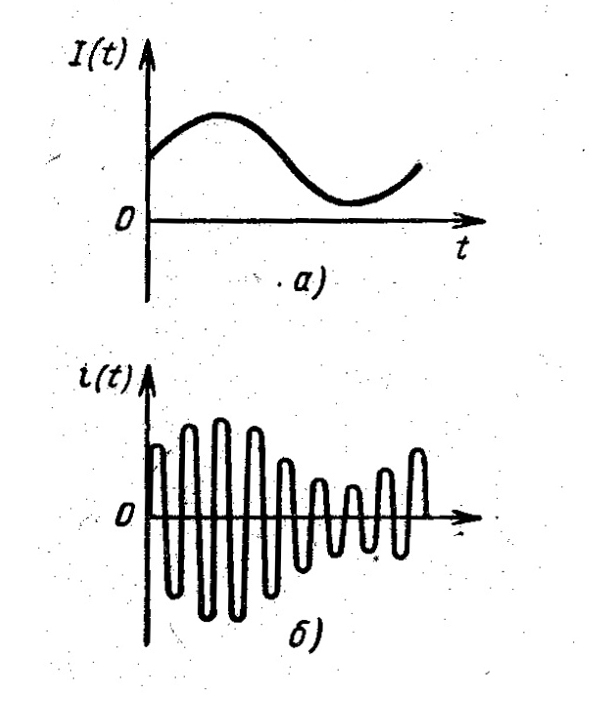
\includegraphics[width=0.5\linewidth]{fig/fig1}
	\caption{Амплитудная модуляция (а - сигнал; б - модулированное колебание, соответствующее сигналу).}
	\label{fig:fig1}
\end{figure}

Если обозначить через $I_{\text{н}}$ амплитуду высокочастотного колебания до
осуществления модуляции и предположить, что во время модуляции изменение амплитуды $I_m$ прямо пропорционально силе звука нашего сигнала, то закон изменения амплитуды тока высокой частоты при модуляции чистым тоном
звуковой частоты $\Omega$ запишется так: 

$$I_{\text{н}}+I_1\cos{\Omega t},$$

\begin{equation}
	i = I_{\text{н}}(1+m\cos{\Omega t})\cos{\omega_0 t},
\end{equation}
где $m=\frac{I_1}{I_{\text{н}}}$ - коэффициент модуляции.

\subsection{Анализ модулированных колебаний}

После несложных преобразований выражение (1) может быть представлено следующим образом: 

\begin{equation}
	i = I_{\text{н}}\cos{\omega_0 t}+mI_{\text{н}}\cos{\Omega t}\cos{\omega_0 t}
\end{equation}
или
\begin{equation}
	i = I_{\text{н}}\cos{\omega_0 t}+\frac12mI_{\text{н}}\cos{(\omega_0+\Omega)t}+\frac12mI_{\text{н}}\cos{(\omega_0-\Omega)t}.
\end{equation}

Из полученного выражения видно, что колебание, модулированное одной звуковой частотой $\Omega$ ($\Omega$— частота модуляции), состоит из трех гармонических колебаний.

Первое колебание частоты $\omega_0$ имеет амплитуду, равную амплитуде колебания до осуществления модуляции; второе и третье колебания частот $\omega_0+\Omega$ и $\omega_0-\Omega$ имеют амплитуды, равные $\frac12mI_{\text{н}}$, т.е. их амплитуды прямо пропорциональны коэффициенту модуляции. Частота $\omega_0$ называется несущей частотой, частоты $\omega_0+\Omega$ и $\omega_0-\Omega$ боковыми частотами.

Спектр модулированных колебаний можно наглядно представить в виде графика, откладывая по горизонтальной оси частоты, а по вертикальной – амплитуды тех колебаний, которые входят в состав модулированного тока. Колебание, модулированное одной звуковой частотой $\Omega$, будет иметь спектр, состоящий из несущей и двух боковых частот (Рис.2а).

\begin{figure}[h!]
	\centering
	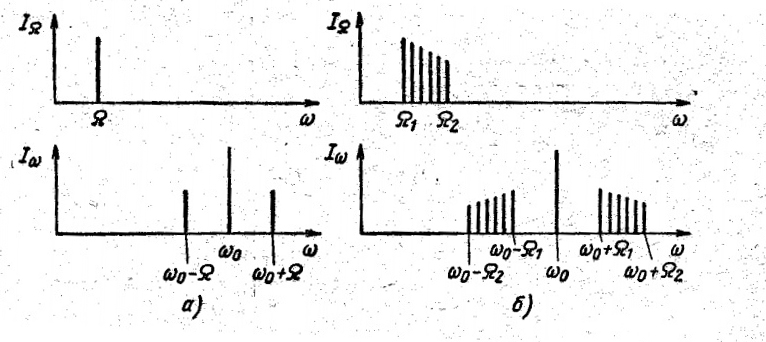
\includegraphics[scale=1.5]{fig/fig2}
	\caption{ Частотные спектры сигналов и колебаний высокой частоты,
	модулированных по амплитуде в соответствии с этими сигналами.}
	\label{fig:fig2}
\end{figure}

Если звуковой сигнал содержит в себе непрерывную полосу частот от $\Omega_1$ до $\Omega_2$, то спектр модулированного колебания будет состоять из несущей частоты и двух боковых полос частот (Рис.2б).

\section{ОДНОПОЛОСНАЯ МОДУЛЯЦИЯ}
\subsection{Принцип действия и основные особенности}

Для передачи информации на дальние и сверхдальние расстояния в настоящее время широко применяются системы связи с одной боковой полосой, обеспечивающие при одинаковой мощности передатчика значительно более высокую надежность связи по сравнению с системами, в которых используется обычная амплитудная модуляция.

Прежде чем перечислить основные преимущества и недостатки систем с одной боковой полосой, кратко остановимся на принципе их работы, в частности на простейшем способе образования однополосного сигнала и его отличии от обычного сигнала с амплитудной модуляцией.

\begin{figure}[H]
	\centering
	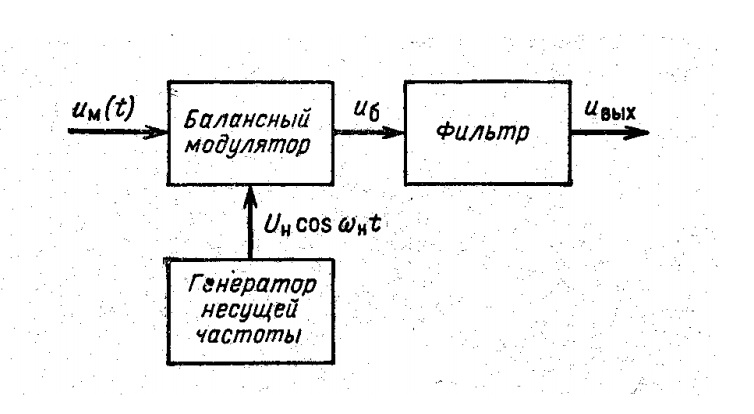
\includegraphics[width=0.5\linewidth]{fig/fig3}
	\caption{ Блок-схема формирования однополосного сигнала.}
	\label{fig:fig3}
\end{figure}

Для образования однополосного сигнала, т. е. сигнала, содержащего только верхнюю или нижнюю боковую полосу, используются балансные модуляторы. Ко входу такого модулятора (Рис.3.) одновременно подводятся напряжение передаваемого сигнала (спектр которого показан на (Рис.4а) и напряжение несущей частоты. На выходе модулятора сохраняются только
верхняя и нижняя боковые полосы (Рис.4б). 

Для получения однополосного сигнала с помощью фильтра вырезается верхняя или нижняя боковая полоса (Рис.4в), которая после усиления в высокочастотном тракте передатчика поступает в антенну и излучается.

Нетрудно видеть, что спектр однополосного сигнала по форме совпадает со спектром исходного модулирующего напряжения, однако он смещен на частоту $\omega_0$ в область более высоких частот. Информация, содержащаяся в одной боковой полосе, является недостаточной для восстановления передаваемого сигнала. Дело в том, что если нам неизвестно значение несущей частоты, то мы не сможем определить частоты передаваемого сигнала.

\begin{figure}[h!]
	\centering
	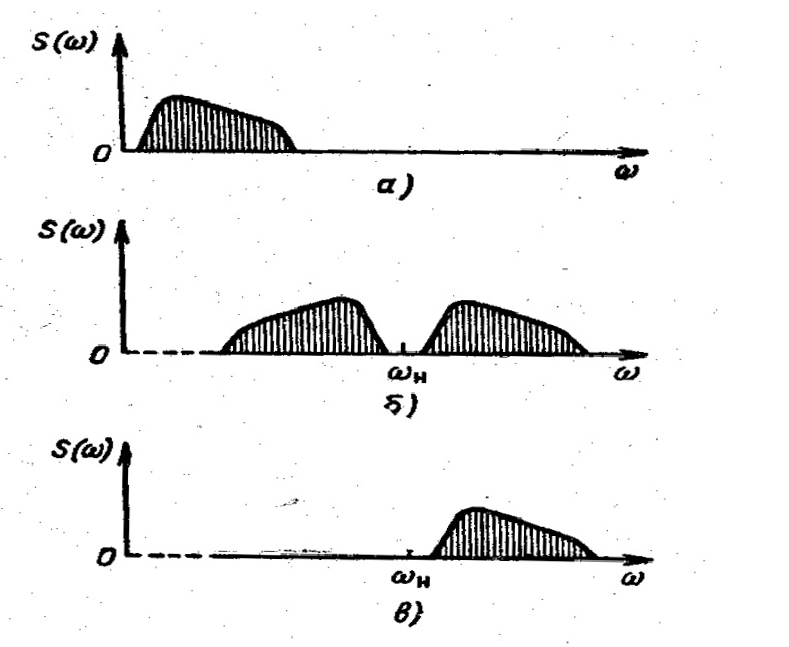
\includegraphics[scale=1.5]{fig/fig4}
	\caption{ Графики спектральной плотности сигналов: а) модулирующего;
б) двухполосного (без несущей); в) однополосного.}
	\label{fig:fig4}
\end{figure}

Таким образом, при приеме однополосного сигнала необходимо в точке приема восстанавливать несущую частоту. Остановимся на некоторых особенностях систем однополосной передачи.

К числу основных преимуществ таких систем по сравнению с обычными
амплитудно-модулированными системами можно отнести:
\begin{enumerate}
	\item устранение из спектра несущей частоты и одной боковой полосы, для
передачи которых в обычных системах затрачивается значительная мощность;
	\item уменьшение полосы частот, занимаемой передатчиком, дающее возможность увеличить число станций, работающих без взаимных помех в заданном диапазоне, и существенно снизить искажение передаваемого сигнала, вызванное селективным «замиранием», которое является следствием неодинаковости условий распространения различных по частоте составляющих
спектра сигнала;
	\item сужение полосы пропускания приемного устройства, позволяющее примерно в два раза снизить мощность помех на входе приемника. 
\end{enumerate}

Говоря об энергетических преимуществах рассматриваемых систем, следует заметить, что при отсутствии модулирующего сигнала (например, при молчании перед микрофоном) передатчик не излучает, в то время как в обычных системах излучается несущая частота. Учитывая, что подобные паузы при радиотелефонной передаче составляют значительную часть времени работы, применение однополосной передачи дает дополнительный, существенный энергетический выигрыш.

Полный энергетический выигрыш по сравнению с системой обычной амплитудной модуляции приблизительно оценивается в 15 — 20 раз. 

К основным недостаткам систем однополосной передачи следует отнести:
\begin{enumerate}
	\item Необходимость обеспечения высокой стабильности частоты передатчика и генератора несущей частоты, восстанавливаемой на приемном конце. Отклонение восстановленной в приемнике несущей частоты от подавленной в передатчике при коммерческой связи обычно не превышает 50 — 100 Гц. Если разница превосходит указанное значение, то резко снижается
разборчивость передаваемой речи. Хорошая разборчивость речи получается, если отклонение не превышает 15 — 20 Гц. Для высококачественного приема музыкальных передач допустимая величина отклонения измеряется единицами и даже долями герца.
	\item Усложнение приемной и передающей аппаратуры, связанное с формированием однополосного сигнала, а также с восстановлением несущей частоты при демодуляции в приемном устройстве. 
\end{enumerate}
Так как к точности восстановленной несущей частоты и строгости ее поддержания постоянной предъявляются высокие требования, то для контроля или автоматической подстройки несущей частоты вместе с однополосным сигналом может передаваться или значительно ослабленная несущая частота или так называемый пилот-сигнал. В ряде случаев оказывается нецелесообразным сохранять несущую частоту во всем тракте формирования однополосного сигнала, а удобнее «замешивать» ее в передаваемый сигнал в выходных каскадах передатчика.

Необходимость достаточно точного восстановления несущей частоты затрудняет использование однополосной связи с быстро летящими объектами, так как при изменении направления движения и скорости объекта вследствие влияния эффекта Доплера наблюдается заметное отклонение частоты принимаемых сигналов от частоты сигналов, излучаемых передатчиком.

При осуществлении однополосной связи с быстролетящими объектами необходимо компенсировать доплеровский сдвиг частоты. Это можно сделать, например, используя автоматическую подстройку частоты по пилот-сигналу.

Для повышения коэффициента полезного действия передатчиков с одной боковой полосой целесообразно формирование однополосного сигнала производить в маломощных каскадах передатчика, а затем усиливать его до необходимого уровня в последующих каскадах передатчика. При этом следует иметь в виду, что при выделении одной боковой полосы из амплитудно-модулированного колебания на выходе фильтра получается колебание с
амплитудно-частотной модуляцией.

Из этого свойства однополосного сигнала следует первая особенность усилительного тракта рассматриваемых передатчиков, а именно недопустимость использования в усилительном тракте каскадов умножения частоты.

Второй важной особенностью усилительного тракта однополосного передатчика являются высокие требования к линейности его амплитудной характеристики. Допустимый уровень нелинейных искажений значительно ниже, чем в обычных передатчиках. Это объясняется тем, что если среднее значение огибающей амплитудно-модулированного сигнала не зависит от характера модулирующего сигнала и определяется амплитудой колебания несущей частоты, то среднее значение огибающей однополосного сигнала зависит от величины модулирующего напряжения и обычно заметно ниже среднего значения амплитудно-модулированного сигнала. Очевидно, что в результате снижения среднего уровня сигнала усиление происходит на нижнем
участке амплитудной характеристики каскадов передатчика, и поэтому для предотвращения сильных искажений необходимо обеспечивать высокую линейность не только основной части амплитудной характеристики усилителя, но и ее начального участка. Так как усилительные каскады передатчика обычно работают с отсечкой анодного тока, т. е. в режиме колебаний 2-го рода, получение высокой линейности начального участка амплитудной характеристики усилителя обычно сопряжено с определенными трудностями и в ряде случаев требует применения специальных, активных элементов, имеющих линейный нижний участок статической характеристики выходного тока. 

Для формирования однополосного сигнала в настоящее время
используются три основных метода: 
\begin{enumerate}
	\item фильтровой;
	\item фазокомпенсационный;
	\item фазофильтровой.
\end{enumerate} 

\subsection{Фильтровой метод}

При высокой несущей частоте в ряде случаев возникают определенные технические трудности выделения только одной боковой полосы.

Действительно, если, например, нижняя граница спектра передаваемого звукового сигнала равна 200 Гц, то нижняя и верхняя боковые полосы будут удалены друг от друга на 400 Гц. При несущей частоте 10 МГц это составит 0,004\%. Разделение столь близко расположенных полос с помощью даже весьма совершенных кварцевых фильтров в этом диапазоне частот чрезвычайно сложно. Чтобы обойти указанное затруднение, обычно используют промежуточное преобразование частоты. 

\begin{figure}[h!]
	\centering
	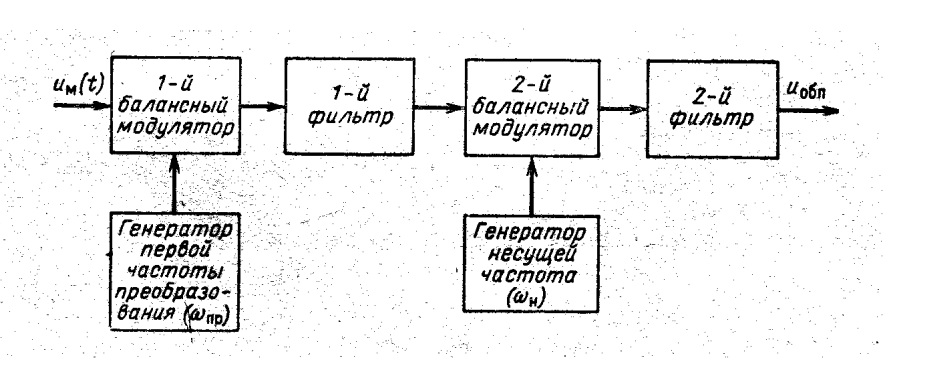
\includegraphics[width=0.8\linewidth]{fig/fig5}
	\caption{ Блок-схема формирования однополосного сигнала фильтровым методом.}
	\label{fig:fig5}
\end{figure}

В качестве примера на Рис.5 приведена блок-схема, а на Рис.6 - спектры сигнала на выходе отдельных элементов схемы, поясняющие формирование однополосного сигнала с одним
промежуточным преобразованием частоты.

\begin{figure}[h!]
	\centering
	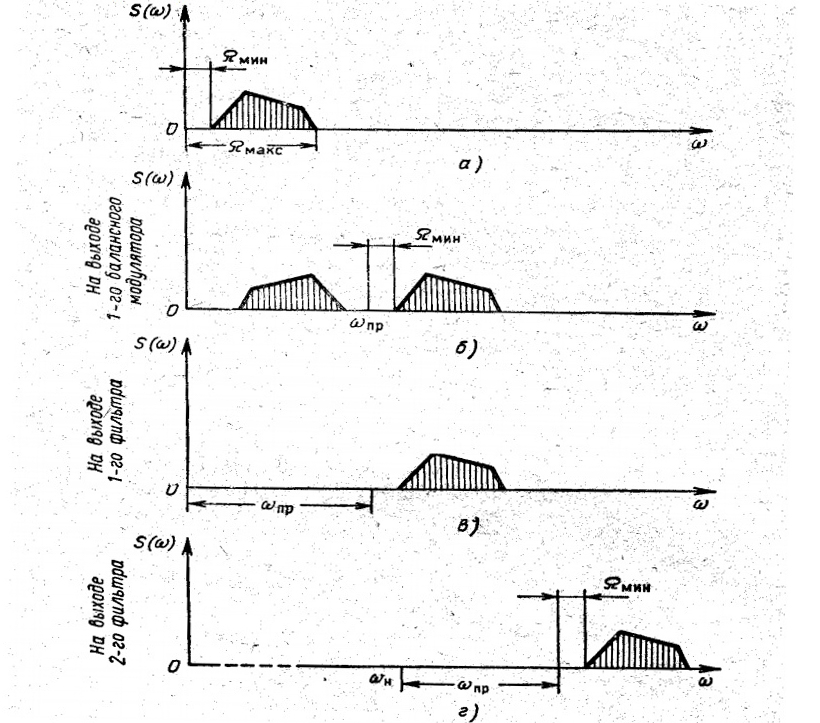
\includegraphics[scale=1.5]{fig/fig6}
	\caption{. Спектры сигнала, поясняющие формирование однополосного сигнала
фильтровым методом: а) исходного; б) на выходе первого модулятора; в) на
выходе первого фильтра; г) на выходе второго фильтра.}
	\label{fig:fig6}
\end{figure}

В данном случае предварительно получается однополосный сигнал на более низкой частоте ($\omega_{\text{пр}}$) по сравнению с несущей, что облегчает фильтрацию одной боковой полосы. Полученный на выходе фильтра сигнал (Рис. 6в), занимающий полосу частот, равную полосе частот входного сигнала, но смещенный по частоте на величину первой промежуточной частоты преобразования $\omega_{\text{пр}}$ (которую иногда называют поднесущей), подается на второй балансный модулятор, на выходе которого получаются две боковые
полосы частот, разнесенные на величину 2($\omega_{\text{пр}}+\Omega_{\text{мин}}$). С выхода балансного модулятора сигнал поступает на второй фильтр для выделения одной боковой полосы.

В данном примере использовано одно промежуточное преобразование. В ряде случаев для получения необходимого подавления несущей и нежелательной боковой полосы приходится использовать несколько подобных преобразований. По этой причине рассмотренный метод получения однополосного сигнала называется в литературе также методом
последовательных преобразований. 

\subsection{Сравнение методов формирования однополосного сигнала}

Различные методы формирования однополосного сигнала имеют свои преимущества и недостатки.

Одним из основных достоинств фазокомпенсационного метода формирования однополосного сигнала по сравнению с фильтровым методом является то, что при его использовании отпадает необходимость применения фильтров с крутым спадом характеристики в области граничных частот. Это, в свою очередь, позволяет использовать в балансных модуляторах непосредственно несущую частоту без многократного частотного преобразования, к которому мы прибегаем в случае подавления одной боковой полосы с помощью фильтров.

Недостатком фазокомпенсационного метода является необходимость использования фазовращателей, обеспечивающих постоянный фазовый сдвиг в широком диапазоне модулирующих частот, а также точный баланс схемы. К недостаткам этого метода относится также применение двух балансных
модуляторов. Указанный недостаток устраняется в многофазных системах, которые позволяют осуществить подавление несущей частоты без балансных модуляторов.

Основным преимуществом фазофильтрового метода перед фильтровым и фазокомпенсационным является отсутствие сложных фазосдвигающих схем, работающих в некотором диапазоне частот, и фильтров с крутыми спадами частотной характеристики. К фильтрам нижних частот, используемым в фазофильтровых схемах, не предъявляются требования резкого спада характеристики в области граничной частоты. 

\section{БАЛАНСНЫЕ МОДУЛЯТОРЫ}

Схема простейшего балансного модулятора приведена на Рис.7. Модулятор состоит из трансформатора $\text{Тр_1}$ на вход которого подается модулирующее напряжение $U_m(t)$ (например, звуковое напряжение в радиотелефонных передатчиках), двух полупроводниковых диодов $\text{Д_1}$ и $\text{Д_1}$, контура LС с катушкой связи $L_{\text{св}}$ с которой снимается выходное напряжение, и высокочастотного трансформатора $\text{Тр_2}$, обеспечивающего подачу напряжения несущей частоты. Конденсаторы $C_0$ шунтируют обмотки трансформатора $\text{Тр_2}$, по несущей частоте. Их сопротивление для модулирующего напряжения должно быть велико. 

\begin{figure}[h!]
	\centering
	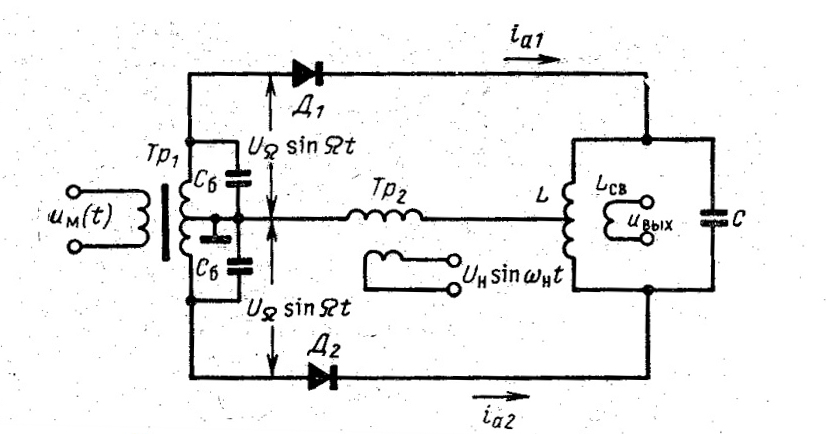
\includegraphics[width=0.8\linewidth]{fig/fig7}
	\caption{Схема балансного модулятора.}
	\label{fig:fig7}
\end{figure}

Предположим, что нелинейные элементы $\text{Д_1}$ и $\text{Д_1}$ имеют одинаковые
характеристики

$$i_a = a_1 + a_2u + a_2u+...,$$ 
%не 3 ли
где $u$ — действующее на элементах напряжение. 
\end{document}
